%% Artículo final — Curso Big Data, Maestría en IA, EPG-UNI
%% Plantilla IEEEtran (conference). Compilar con: pdflatex -> bibtex -> pdflatex x2
\documentclass[conference]{IEEEtran}

\usepackage[utf8]{inputenc}
\usepackage[T1]{fontenc}
% La distribución TeX local no incluye Courier (pcr); usar la typewriter de CM.
\renewcommand{\ttdefault}{cmtt}
\usepackage[spanish,es-noshorthands]{babel}
\usepackage{graphicx}
\usepackage{amsmath}
\usepackage{booktabs}
\usepackage{url}
\usepackage{xcolor}
\usepackage[hidelinks]{hyperref}

\graphicspath{{../figures/}{./figures/}}

\begin{document}

\title{Comparación de algoritmos de aprendizaje automático distribuido para la
predicción de propina baja en viajes de taxi de Nueva York con Apache Spark MLlib}

\author{\IEEEauthorblockN{Niels Pacheco\IEEEauthorrefmark{1}}
\IEEEauthorblockA{\IEEEauthorrefmark{1}Escuela de Posgrado, Universidad Nacional de Ingeniería\\
Maestría en Inteligencia Artificial --- Curso de Big Data\\
Lima, Perú\\
E-mail: nielspacheco1997@gmail.com}
\thanks{Documento de proyecto final individual del curso de Big Data.}}

\maketitle

\begin{abstract}
El crecimiento de los registros operativos del transporte urbano plantea el reto
de aplicar aprendizaje automático sobre volúmenes que exceden la capacidad de una
sola máquina con herramientas tradicionales. Este trabajo formula una pregunta de
investigación de naturaleza comparativa: ¿qué algoritmo de clasificación
distribuida ofrece el mejor compromiso entre desempeño predictivo y costo
computacional para predecir, sobre decenas de millones de viajes de taxi de Nueva
York, si un viaje pagado con tarjeta dejará una propina baja? Utilizando seis
meses de los registros públicos de la NYC Taxi and Limousine Commission
(19{,}5 millones de viajes crudos, 14{,}9 millones tras depuración) y la
biblioteca Apache Spark MLlib, se comparan cuatro clasificadores (regresión
logística, árbol de decisión, random forest y gradient-boosted trees) bajo un
fuerte desbalance de clases ($\approx$9{,}7:1), todos con ponderación de clases.
Los resultados muestran que la \emph{accuracy} es engañosa en este escenario: un
clasificador trivial alcanzaría un 90{,}6\,\% de exactitud con recall nulo sobre la
clase de interés, mientras que los modelos ponderados recuperan entre el 50\,\% y
el 64\,\% de los viajes de propina baja. El gradient-boosted trees logra el mejor
desempeño predictivo (AUC = 0{,}686 y recall de la minoría = 0{,}64) pero al mayor
costo de cómputo; el random forest ofrece un AUC casi equivalente (0{,}680) en la
mitad del tiempo, y la regresión logística es la alternativa más eficiente.
Adicionalmente, dos experimentos de escalabilidad evidencian un crecimiento
sublineal del tiempo de entrenamiento con el volumen (20$\times$ datos
$\rightarrow$ 5$\times$ tiempo) y un \emph{speedup} de 4{,}71$\times$ al pasar de 1
a 8 núcleos, consistente con la ley de Amdahl. Se concluye que, bajo desbalance, la
elección del algoritmo debe guiarse por el AUC y el recall de la minoría,
sopesando el costo computacional, y no por la exactitud.
\end{abstract}

\begin{IEEEkeywords}
Big Data; Apache Spark; MLlib; aprendizaje distribuido; desbalance de clases;
escalabilidad; NYC Taxi.
\end{IEEEkeywords}

\section{Introducción}
La generación masiva de datos por sistemas de transporte, sensores y plataformas
digitales ha consolidado el paradigma de Big Data, caracterizado por las llamadas
cinco V: volumen, velocidad, variedad, veracidad y valor~\cite{gandomi2015beyond}.
Cuando el volumen de los datos supera la memoria y el cómputo de un único nodo,
distribuir el procesamiento se vuelve inevitable. Apache Spark se ha establecido
como el motor de referencia para este
tipo de cargas gracias a su modelo de cómputo en memoria y a su biblioteca de
aprendizaje automático escalable, MLlib~\cite{zaharia2016spark,meng2016mllib}.

Los registros de viajes de taxi de la ciudad de Nueva York constituyen un caso de
estudio representativo: cada mes se publican millones de viajes con información
espacial, temporal y económica. Sobre ellos es posible plantear problemas de valor
directo para el negocio del transporte, como anticipar la propina que recibirá un
conductor. Para quien maneja el taxi, la propina representa una fracción
apreciable de su ingreso; poder anticiparla ayudaría a diseñar incentivos, a
organizar mejor el despacho y a entender el comportamiento del pasajero.

Este trabajo aborda una tarea de clasificación binaria con relevancia práctica y
con una propiedad estadística que el curso enfatizó reiteradamente: el desbalance
de clases. Se define como clase positiva el viaje con \emph{propina baja} (inferior
al 10\,\% de la tarifa), que resulta minoritario. Más que construir un clasificador
puntual, el trabajo compara de forma controlada cuatro algoritmos distribuidos y
mide cómo escala el sistema, recorriendo el ciclo de vida completo del dato
(ingesta, procesamiento distribuido, modelado y visualización) estudiado a lo
largo del curso.

\section{Estado del arte y trabajos relacionados}
El procesamiento distribuido de datos masivos tiene su antecedente en el modelo
MapReduce~\cite{dean2008mapreduce}, posteriormente superado en eficiencia por
Apache Spark, que evita la materialización en disco entre etapas y unifica el
procesamiento por lotes, en flujo y de aprendizaje automático~\cite{zaharia2016spark}.
MLlib aporta implementaciones distribuidas de los algoritmos clásicos de
clasificación, regresión y \emph{clustering} sobre la API de DataFrames y
\emph{pipelines}~\cite{meng2016mllib}. Estudios comparativos de herramientas de
aprendizaje sobre el ecosistema Hadoop sitúan a Spark MLlib como una de las
opciones más maduras para aprendizaje a gran escala~\cite{landset2015survey}.

El aprendizaje con clases desbalanceadas es un problema ampliamente
estudiado~\cite{he2009imbalanced}. Las estrategias habituales incluyen el
remuestreo sintético de la clase minoritaria mediante SMOTE~\cite{chawla2002smote},
el aprendizaje sensible al costo~\cite{elkan2001costsensitive} y la ponderación de
instancias. En el contexto de Big Data, el remuestreo introduce retos adicionales
de escalabilidad, pues altera el volumen de datos que debe distribuirse y
procesarse~\cite{fernandez2017imbalancedbigdata}. Por ello, en este trabajo se
prefiere la ponderación de clases, que no incrementa el tamaño del conjunto.

Entre los algoritmos comparados, random forest~\cite{breiman2001randomforests} y
el \emph{gradient boosting}~\cite{friedman2001greedy}, popularizado a gran escala
por XGBoost~\cite{chen2016xgboost}, representan dos familias de ensambles con
compromisos distintos entre sesgo, varianza y costo. La evaluación bajo desbalance
exige métricas robustas; el análisis ROC y el área bajo la curva (AUC) son el
estándar al ser insensibles a la proporción de clases~\cite{fawcett2006roc}.
Finalmente, trabajos previos sobre los datos de taxis de Nueva York han abordado el
análisis de demanda y la predicción de duración de viajes con enfoques de Big Data
y \emph{boosting}~\cite{yu2021bigdatataxi,poongodi2022nyc}, aunque la predicción de
propina baja como problema de clasificación desbalanceada ha recibido menos
atención.

\section{Problema de investigación}
Se plantea la siguiente pregunta de investigación:

\begin{quote}
\emph{Sobre decenas de millones de viajes de taxi de Nueva York, ¿qué clasificador
distribuido de Spark MLlib ofrece el mejor compromiso entre desempeño predictivo
(medido con métricas robustas al desbalance) y costo computacional, para predecir
si un viaje pagado con tarjeta dejará una propina baja?}
\end{quote}

De ella se derivan tres preguntas específicas: (i) ¿cómo se comportan regresión
logística, árbol de decisión, random forest y GBT en AUC, F1 y recall de la clase
minoritaria una vez aplicado el manejo de desbalance?; (ii) ¿cuál es el costo de
entrenamiento de cada uno?; y (iii) ¿cómo escala el tiempo de cómputo al aumentar
el volumen de datos y el número de núcleos del procesamiento distribuido?

\section{Metodología}
La solución sigue el ciclo de vida del dato resumido en la
Fig.~\ref{fig:arq}. Cada etapa se asocia a la dimensión de Big Data que aborda.

\begin{figure*}[t]
\centering
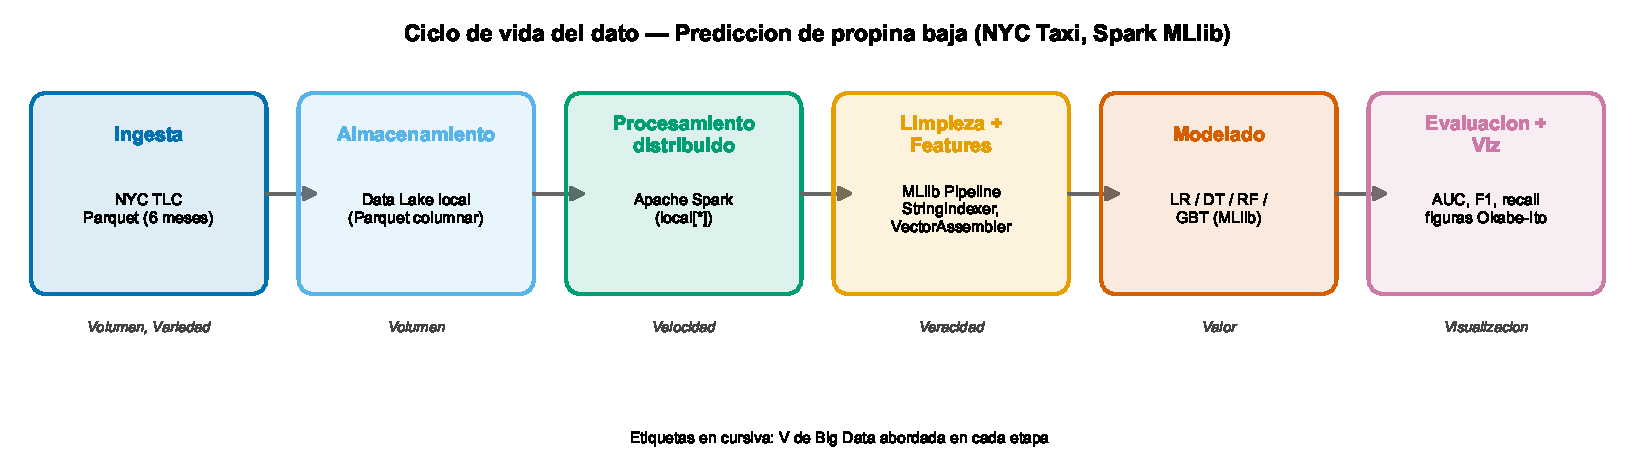
\includegraphics[width=0.95\textwidth]{fig7_arquitectura.pdf}
\caption{Arquitectura del ciclo de vida del dato. La ingesta normaliza el esquema
de los Parquet mensuales; Spark realiza el procesamiento distribuido; un
\emph{pipeline} de MLlib construye las variables y entrena los modelos; la
evaluación reporta métricas robustas al desbalance y produce las visualizaciones.}
\label{fig:arq}
\end{figure*}

\subsection{Infraestructura}
Los experimentos se ejecutaron con Apache Spark 3.5.3 sobre Java 11 y Python 3.11,
en modo local (\texttt{local[*]}) en una máquina con 16 núcleos y 68\,GB de RAM
física, asignando 24\,GB a la memoria del \emph{driver} de Spark. El
modo local instancia un \emph{executor} multihilo que simula el paralelismo de un
clúster, lo que garantiza reproducibilidad sin costos de nube; el mismo código
migra sin cambios a un clúster gestionado como AWS EMR o Databricks.

\subsection{Conjunto de datos y depuración}
Se emplearon los registros públicos de \emph{Yellow Taxi} de la NYC Taxi and
Limousine Commission correspondientes a los seis primeros meses de 2023, en formato
Apache Parquet. Dado que el esquema físico de algunas columnas varía entre meses
(p.\,ej.\ \texttt{passenger\_count} como entero o real), la ingesta lee cada archivo
y castea las columnas a tipos canónicos antes de unirlos, evitando errores de
fusión de esquemas. La depuración descartó registros con valores no plausibles:
solo viajes pagados con tarjeta de crédito (la propina en efectivo no se registra),
con tarifa y distancia positivas y acotadas, entre uno y seis pasajeros, duración
entre 1 y 180 minutos y velocidad media menor a 100\,mph. De los 19{,}5 millones de
viajes crudos se conservaron 14{,}9 millones.

\subsection{Definición de la etiqueta y variables}
La etiqueta binaria marca como positivo (1) el viaje con \emph{propina baja},
definida como $\textit{tip\_amount}/\textit{fare\_amount} < 0{,}10$. Para evitar
\emph{fuga de objetivo} se excluyeron explícitamente como predictores la propina y
el importe total (que la contiene por construcción). El vector de variables combina
catorce atributos numéricos (distancia, número de pasajeros, duración, velocidad
media, tarifa, recargos, hora del día, indicadores de fin de semana y de
madrugada, y las zonas de origen y destino) con dos atributos categóricos, el día
de la semana y el código de tarifa, codificados con \emph{one-hot}. La construcción del
vector reproduce el patrón canónico de MLlib: \texttt{StringIndexer},
\texttt{OneHotEncoder} y \texttt{VectorAssembler} encadenados en un
\texttt{Pipeline}.

\subsection{Manejo del desbalance}
La clase minoritaria representa el 9{,}36\,\% de los viajes, un desbalance de
9{,}69:1 (Fig.~\ref{fig:balance}). Sin tratamiento, un clasificador trivial que
prediga siempre ``propina normal'' alcanzaría un 90{,}6\,\% de exactitud y 0\,\%
de recall sobre la clase de interés. Se aplicó ponderación de instancias: a cada
viaje de la clase $c$ se le asigna un peso $w_c = N / (2\,N_c)$, de modo que ambas
clases contribuyen por igual a la función de pérdida. Esta técnica, soportada
nativamente por los cuatro clasificadores en Spark~3.x mediante el parámetro
\texttt{weightCol}, garantiza una comparación equitativa y no incrementa el volumen
de datos, a diferencia del remuestreo.

\subsection{Modelos y evaluación}
Se compararon cuatro clasificadores de \texttt{pyspark.ml}: regresión logística
(línea base lineal), árbol de decisión (profundidad 10), random forest (50 árboles,
profundidad 10) y gradient-boosted trees (50 iteraciones, profundidad 6). La
comparación se realizó sobre una muestra de dos millones de viajes dividida en
80\,\% para entrenamiento (1{,}60\,M) y 20\,\% para prueba (0{,}40\,M), idéntica
para todos los modelos. Se reportan el AUC-ROC mediante
\texttt{BinaryClassificationEvaluator}, y la exactitud, precisión, recall y F1
ponderados mediante \texttt{MulticlassClassificationEvaluator}, además del recall
de la clase minoritaria calculado explícitamente.

\subsection{Experimentos de escalabilidad}
Se diseñaron dos benchmarks. En la \emph{escalabilidad de datos} se fijó el
paralelismo y se entrenó la regresión logística sobre fracciones crecientes (de
0{,}75\,M a 14{,}9\,M de filas), midiendo el tiempo de ajuste. En la
\emph{escalabilidad fuerte} se fijó el volumen en tres millones de viajes y se
varió el número de núcleos del \emph{executor} (1, 2, 4 y 8), midiendo el
\emph{speedup} respecto a un núcleo. En ambos casos los datos se materializaron en
caché antes de cronometrar para no contabilizar la lectura perezosa.

\section{Experimentos y resultados}

\subsection{Análisis exploratorio}
El volumen mensual se mantiene estable en torno a 2{,}5 millones de viajes
(Fig.~\ref{fig:volumen}), confirmando la magnitud del problema. La tasa de propina
baja presenta un patrón temporal claro, con mayor incidencia en la madrugada
(donde alcanza $\approx$17{,}8\,\% frente al $\approx$9{,}4\,\% global), lo
que sugiere que las variables temporales aportan señal. No obstante, el
considerable solapamiento de las distribuciones de las variables operativas entre
ambas clases anticipa que la tarea es intrínsecamente difícil.

\begin{figure}[t]
\centering
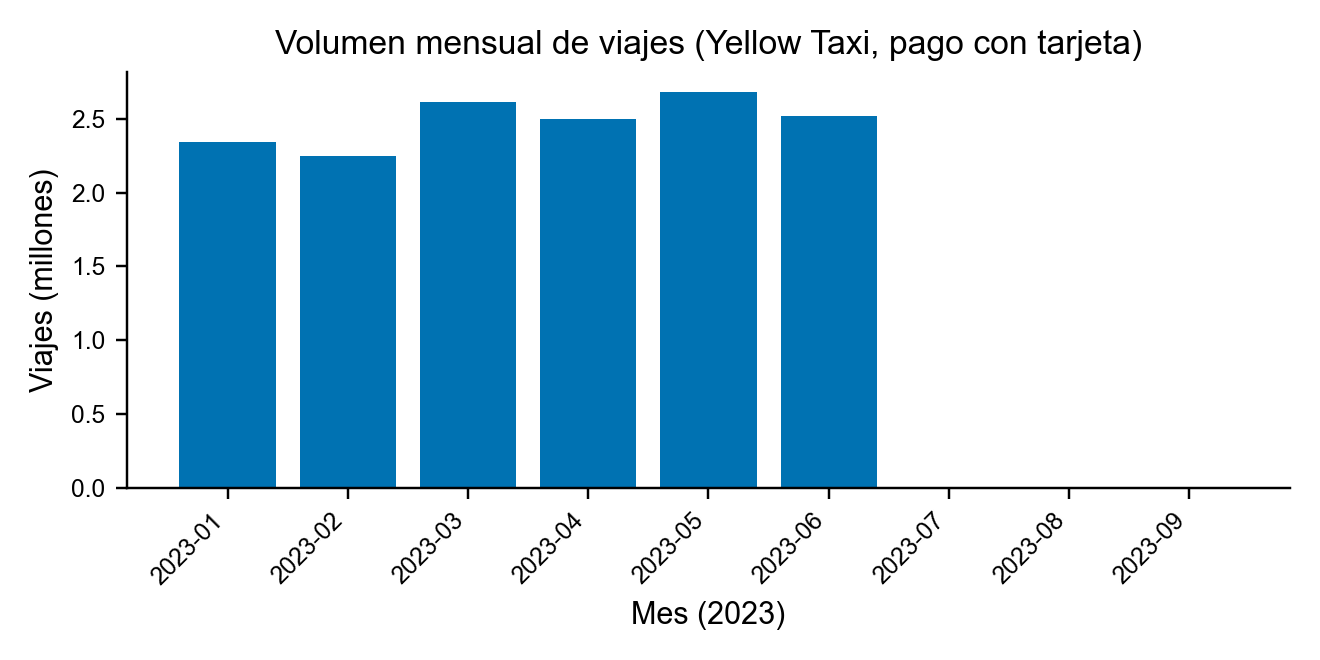
\includegraphics[width=0.85\columnwidth]{fig1_volumen_mensual.png}
\caption{Volumen mensual de viajes pagados con tarjeta (2023). El sistema procesa
del orden de 2{,}5 millones de registros por mes.}
\label{fig:volumen}
\end{figure}

\begin{figure}[t]
\centering
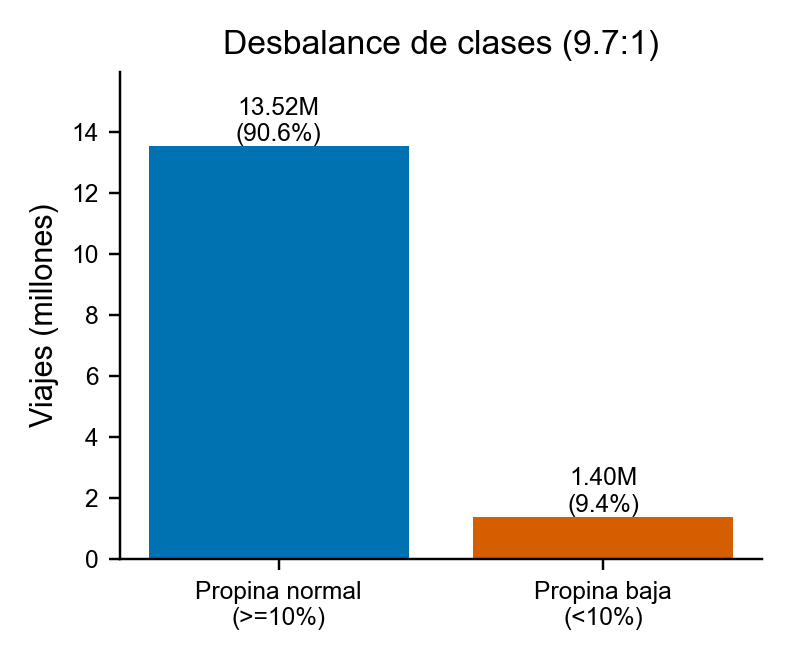
\includegraphics[width=0.74\columnwidth]{fig3_balance_clases.png}
\caption{Desbalance de clases: la propina baja es minoritaria (9{,}4\,\%), con una
razón de 9{,}7:1 frente a la clase mayoritaria.}
\label{fig:balance}
\end{figure}

\subsection{Comparación de modelos}
La Tabla~\ref{tab:modelos} y la Fig.~\ref{fig:modelos} resumen el desempeño de los
cuatro modelos entrenados con ponderación de clases. Antes de compararlos conviene
fijar una referencia: un clasificador trivial que prediga siempre la clase
mayoritaria (``propina normal'') alcanzaría una exactitud de 90{,}6\,\% pero un
recall nulo sobre la clase de interés. Este contraste es la primera evidencia de
que la exactitud es una métrica engañosa bajo desbalance: tras la ponderación, la
exactitud de los modelos desciende al rango 0{,}61--0{,}69 mientras que su recall
de la minoría asciende a 0{,}50--0{,}64, lo que indica que ahora sí detectan los
viajes de propina baja en lugar de ignorarlos.

\begin{table}[t]
\caption{Desempeño en el conjunto de prueba (0{,}40\,M de viajes), con ponderación
de clases en los cuatro modelos. Recall+ es el recall de la clase minoritaria
(propina baja). La exactitud (Acc.) se reporta por completitud, no como criterio de
selección. En negrita, el mejor valor de cada columna salvo Acc.}
\label{tab:modelos}
\centering
\renewcommand{\arraystretch}{1.15}
\begin{tabular}{lccccc}
\toprule
Modelo & AUC & F1 & Acc. & Recall+ & Tiempo (s) \\
\midrule
Regresión logística & 0{,}656 & \textbf{0{,}753} & 0{,}691 & 0{,}501 & 9{,}0 \\
Árbol de decisión   & 0{,}541 & 0{,}690 & 0{,}609 & \textbf{0{,}637} & \textbf{3{,}1} \\
Random forest       & 0{,}680 & 0{,}720 & 0{,}646 & 0{,}598 & 27{,}6 \\
GBT                 & \textbf{0{,}686} & 0{,}702 & 0{,}623 & \textbf{0{,}637} & 49{,}2 \\
\bottomrule
\end{tabular}
\end{table}

\begin{figure}[t]
\centering
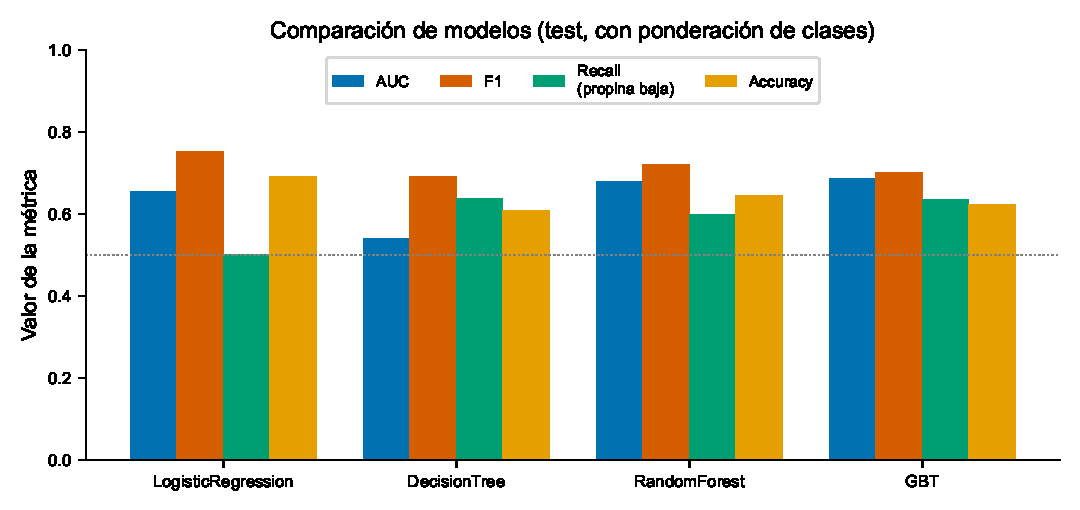
\includegraphics[width=\columnwidth]{fig8_comparacion_modelos.pdf}
\caption{Comparación de modelos con ponderación de clases. Los ensambles (random
forest y GBT) logran el mayor AUC; el árbol y el GBT, el mayor recall de la clase
minoritaria. La exactitud no refleja la utilidad real bajo desbalance.}
\label{fig:modelos}
\end{figure}

El gradient-boosted trees obtiene el mejor desempeño predictivo, con el mayor AUC
(0{,}686) y, junto al árbol, el mayor recall de la minoría (0{,}637), pero a costa
del mayor tiempo de entrenamiento (49{,}2\,s). El random forest alcanza un AUC
prácticamente equivalente (0{,}680; la diferencia de 0{,}006 frente al GBT es
despreciable con un único particionado) y un recall de 0{,}60 en aproximadamente la
mitad del tiempo (27{,}6\,s), por lo que constituye un compromiso atractivo. La
regresión logística es la opción más eficiente entre los modelos de AUC
competitivo: cinco veces más rápida que el GBT (9{,}0\,s) con un AUC de 0{,}656. El
árbol de decisión es el más veloz (3{,}1\,s) y empata en recall, pero su AUC es el
más bajo (0{,}541), señal de una capacidad de \emph{ranking} pobre. La
Fig.~\ref{fig:tradeoff} sitúa cada modelo en el plano desempeño--costo y hace
explícito el frente de compromiso.

\begin{figure}[t]
\centering
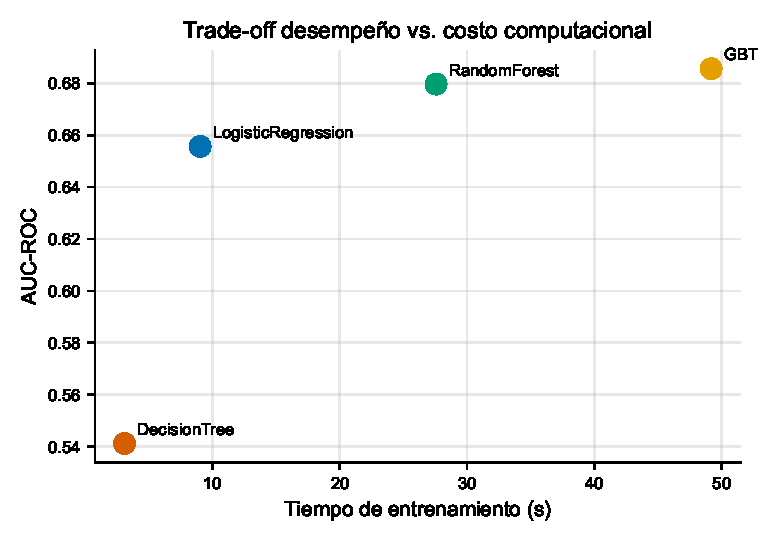
\includegraphics[width=0.82\columnwidth]{fig9_tradeoff.pdf}
\caption{Compromiso entre AUC y tiempo de entrenamiento. El GBT maximiza el AUC al
mayor costo; el random forest ofrece un AUC casi igual a la mitad del tiempo; la
regresión logística es el punto más eficiente.}
\label{fig:tradeoff}
\end{figure}

\subsection{Escalabilidad}
El tiempo de entrenamiento de la regresión logística crece de forma sublineal con
el volumen: multiplicar los datos por veinte (de 0{,}75\,M a 14{,}9\,M) solo
multiplica el tiempo por cinco (de 6{,}1 a 30{,}3\,s), gracias al paralelismo de
datos de Spark (Fig.~\ref{fig:dscaling}). El experimento de escalabilidad fuerte
(Fig.~\ref{fig:strong}) muestra un \emph{speedup} de 1{,}93$\times$ con dos núcleos
(próximo al ideal) que se aleja progresivamente de la recta ideal hasta
4{,}71$\times$ con ocho núcleos. Este comportamiento sublineal es consistente con
la ley de Amdahl~\cite{amdahl1967validity}: la fracción serial del trabajo y los
costos de coordinación limitan la ganancia marginal de cada núcleo adicional.

\begin{figure}[t]
\centering
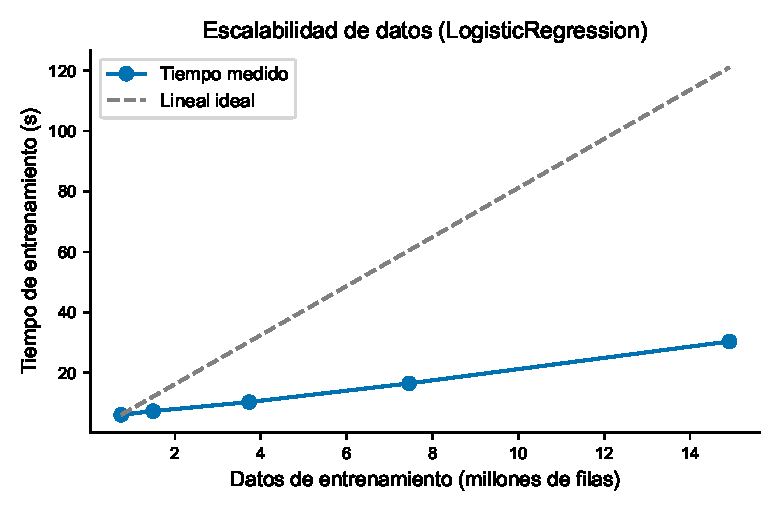
\includegraphics[width=0.82\columnwidth]{fig10_escalabilidad_datos.pdf}
\caption{Escalabilidad de datos: el tiempo de entrenamiento crece por debajo de la
referencia lineal al aumentar el volumen.}
\label{fig:dscaling}
\end{figure}

\begin{figure}[t]
\centering
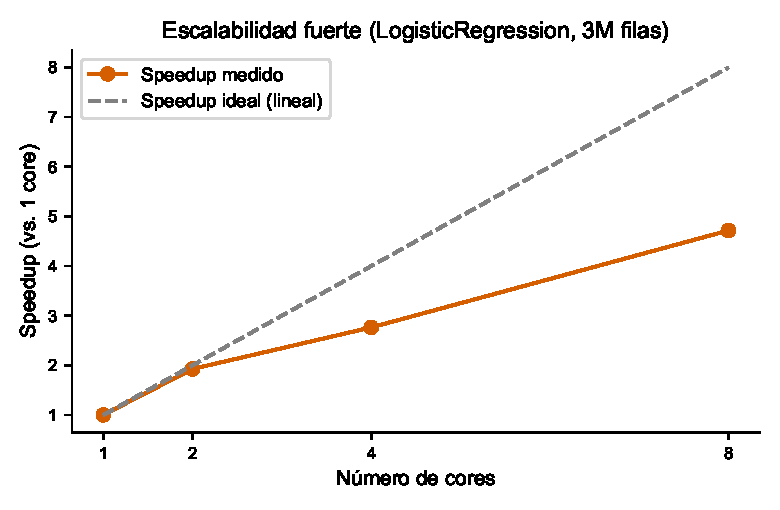
\includegraphics[width=0.82\columnwidth]{fig11_escalabilidad_fuerte.pdf}
\caption{Escalabilidad fuerte: \emph{speedup} frente al número de núcleos. La
separación creciente respecto a la recta ideal refleja la ley de Amdahl.}
\label{fig:strong}
\end{figure}

\section{Discusión}
Los resultados permiten responder la pregunta de investigación, y la respuesta
depende del criterio de decisión. Si se prioriza el desempeño predictivo, el
gradient-boosted trees es la mejor opción, con el mayor AUC y el mayor recall de la
minoría, aunque al mayor costo de cómputo. Si se incorpora el costo, el random
forest emerge como el compromiso más equilibrado: un AUC estadísticamente
indistinguible del GBT (diferencia de 0{,}006 con un único particionado, sin
prueba de significancia) en la mitad del tiempo. Si el costo es la restricción
dominante, la regresión logística ofrece un AUC competitivo a una quinta parte del
tiempo del GBT. La lección metodológica central, sin embargo, es transversal a la
elección del modelo: la exactitud no es una métrica honesta bajo desbalance. Un
clasificador trivial alcanzaría un 90{,}6\,\% de exactitud sin detectar un solo
viaje de propina baja; los modelos resultan útiles solo cuando se observan el AUC y
el recall de la clase minoritaria y se aplica ponderación de
clases~\cite{he2009imbalanced,fawcett2006roc}.

El desempeño absoluto es moderado (AUC en torno a 0{,}68), lo que indica que la
propina es difícil de predecir a partir de las variables operativas del viaje. Esto
es coherente con la naturaleza del fenómeno: la propina depende de factores que el
registro administrativo no captura, como la interacción con el conductor, la
satisfacción del pasajero o las preferencias individuales. La señal disponible es
real pero limitada, y ningún algoritmo puede extraer información que los datos no
contienen.

Desde la perspectiva de las cinco V, el trabajo ejercita el \emph{volumen} (decenas
de millones de registros), la \emph{variedad} (atributos espaciales, temporales y
económicos), la \emph{veracidad} (la decisión de restringirse a pagos con tarjeta
para asegurar la fiabilidad de la propina) y el \emph{valor} (anticipar la
recompensa del conductor). La escalabilidad observada confirma que la arquitectura
es apropiada para el crecimiento del volumen.

\section{Limitaciones}
El estudio presenta limitaciones que delimitan la validez de sus conclusiones.
Primero, la restricción a pagos con tarjeta introduce un sesgo de selección: el
comportamiento de propina en efectivo, no registrado, podría diferir. Segundo, la
comparación se basa en un único particionado entrenamiento/prueba con una semilla
fija; no se calcularon intervalos de confianza ni pruebas de significancia, por lo
que las diferencias pequeñas de AUC entre los mejores modelos (del orden de
0{,}006) deben interpretarse como equivalencia práctica y no como superioridad.
Tercero, la ejecución en modo local no captura los costos de red y \emph{shuffle}
entre nodos de un clúster real, por lo que las curvas de escalabilidad deben leerse
como una cota optimista. Cuarto, no se realizó una búsqueda exhaustiva de
hiperparámetros, de modo que los desempeños reportados son representativos pero no
necesariamente óptimos.

\section{Conclusiones}
Se comparó de forma controlada el desempeño y el costo de cuatro clasificadores
distribuidos de Spark MLlib para predecir la propina baja en viajes de taxi de
Nueva York, sobre 14{,}9 millones de registros y bajo un desbalance de 9{,}7:1. La
experiencia con el análisis de los datos confirma tres aprendizajes. Primero, en
problemas desbalanceados la elección del modelo debe guiarse por el AUC y el recall
de la minoría, y no por la exactitud, que un clasificador trivial inflaría hasta el
90{,}6\,\% sin utilidad alguna. Segundo, no existe un único
modelo dominante: el GBT maximizó el desempeño, el random forest ofreció el mejor
equilibrio desempeño--costo y la regresión logística fue la más eficiente, de modo
que la decisión depende del presupuesto de cómputo. Tercero, los experimentos de
escalabilidad confirmaron empíricamente las ventajas del procesamiento distribuido
y sus límites teóricos según la ley de Amdahl. Como trabajo futuro se plantea incorporar técnicas de remuestreo
distribuido y aprendizaje sensible al costo, enriquecer las variables con datos
contextuales (clima, eventos, tráfico) y desplegar el \emph{pipeline} en un clúster
real para validar la escalabilidad horizontal a escala de múltiples nodos.

% ieeetr: estilo IEEE numérico incluido en toda distribución TeX. En Overleaf
% puede cambiarse a IEEEtran para el formato exacto de las plantillas IEEE.
\bibliographystyle{ieeetr}
\bibliography{refs}

\end{document}
